\noindent Se basa en conjuntos geométricos, áreas y subconjuntos en un espacio acotado, donde a cada subconjunto de $\Omega$ con área bien definida, se le asigna una probabilidad que es la proporción entre su área y el área de $\Omega$.

\begin{equation}
    P(A) = \frac{\text{Área de A}}{\text{Área de $\Omega$}} 
\end{equation}
\\
\noindent\textbf{Ejemplo:} Imagina que vas a tomar un autobús. El autobús llaga entre las 12 pm y la 1 pm. Es decir, los tiempos de llegada tuyo y del autobús son valores $x \in [0, 60]$. Además, supongamos que cuando el autobús llega, permanece en la parada 5 minutos antes de irse; y cuando tú llegas, esperas 20 minutos antes de irte si el autobús no llega. ¿Cuál es la probabilidad de que tomes el autobús? \\

\noindent\textbf{Solución:} En este caso podemos considerar nuestro espacio muestral de la siguiente manera

\begin{equation*}
    \Omega = [0,60] \times [0,60] = \{(x,y) \in \mathbb{R}^{2} | x \in [0,60] \wedge y \in [0,60]\}
\end{equation*}

\begin{figure}[H] 
    \centering 
    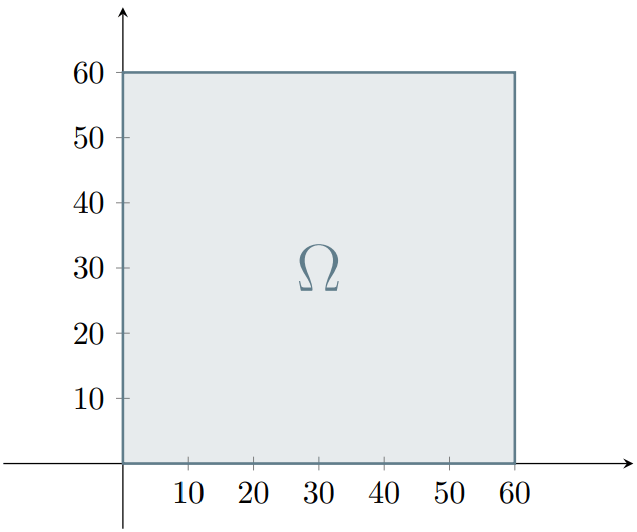
\includegraphics[width=0.4\textwidth]{1 Introducción/1.1 Tipos de probabilidad/1.1 Imágenes/Probabilidad geometrica 2.png}
    \caption{Espacio muestral $\Omega$}
\end{figure}

\noindent Ahora, como el autobús se espera 5 minutos después de llegar, tu tiempo de llegada $x$ debe ser menor o igual a $y+5$, es decir, $a \leq y+5$. Podemos tomar a este evento como el evento $A$ y se representaría de la siguiente manera

\begin{equation*}
    A = \{(x,y) \in \Omega | x-5 \leq y\}
\end{equation*}

\begin{figure}[H] 
    \centering 
    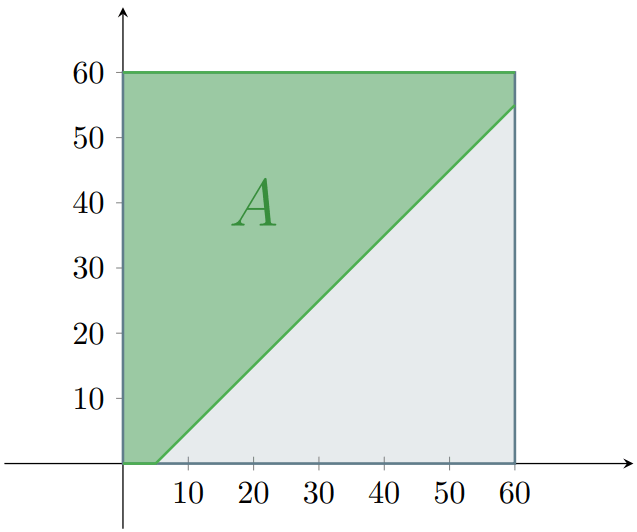
\includegraphics[width=0.4\textwidth]{1 Introducción/1.1 Tipos de probabilidad/1.1 Imágenes/Probabilidad geometrica 3.png}
    \caption{Evento $A$}
\end{figure}

\noindent Por otra parte, tu esperas el autobús por 20 minutos, por lo que $x \geq y-20$, entonces

\begin{equation*}
    B = \{(x,y) \in \Omega | y \leq x+20\}
\end{equation*}

\begin{figure}[H] 
    \centering 
    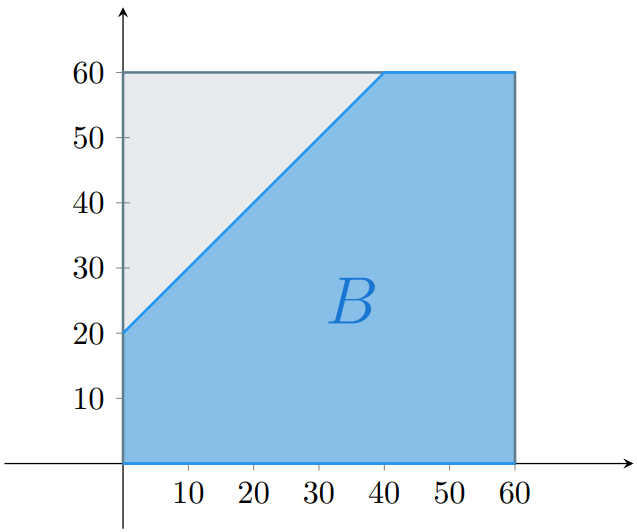
\includegraphics[width=0.4\textwidth]{1 Introducción/1.1 Tipos de probabilidad/1.1 Imágenes/Probabilidad geometrica 4.png}
    \caption{Evento $B$}
\end{figure}

\noindent La intersección de ambas regiones representa cuando tú y el autobús coinciden.

\begin{figure}[H] 
    \centering 
    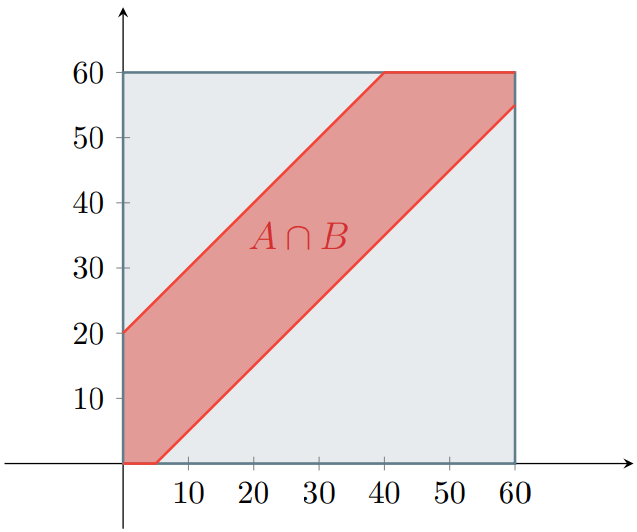
\includegraphics[width=0.4\textwidth]{1 Introducción/1.1 Tipos de probabilidad/1.1 Imágenes/Probabilidad geometrica 5.png}
    \caption{$A \cap B$}
\end{figure}

\noindent Notemos que gráficamente $(A \cap B)^{c}$ forma dos triangulos de área $40^{2}/2$ y $55^{2}/2$

\begin{figure}[H] 
    \centering 
    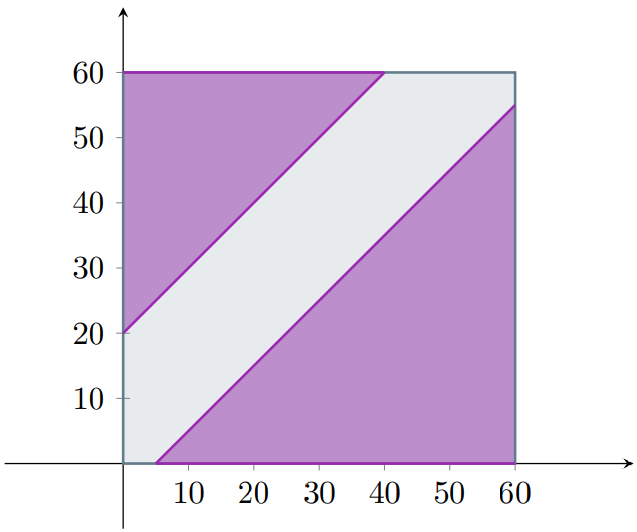
\includegraphics[width=0.4\textwidth]{1 Introducción/1.1 Tipos de probabilidad/1.1 Imágenes/Probabilidad geometrica 6.png}
    \caption{Evento $A$}
\end{figure}

Por lo que podemos calcular la probabilidad de $A \cap B$ como:

\begin{equation*}
    \begin{split}
        P(A \cap B) & = P(\Omega) - P((A \cap B)^{c}) \\
        & = 1 - \left(\frac{\frac{40^{2}}{2}+\frac{55^{2}}{2}}{60^{2}}\right) \\
        & = 1- \frac{4625}{7200} \\
        & = \frac{103}{288}
    \end{split}
\end{equation*}
